% Generator: hand-authored TikZ schematic; coordinates are not to scale.
% Source: fixed 2006 Liaoning science candidate PDF, source ID
% src-db3cbfe3d2c96ec3cbe88c45ad7986cf79f4899fd76a3a73b7c64721f0e67569,
% SHA-256 f680814a4fc5835d805772711f91c5921f12fb92b1740b9c0e9279fa6def427a,
% PDF page 1, printed page 308, Q18.
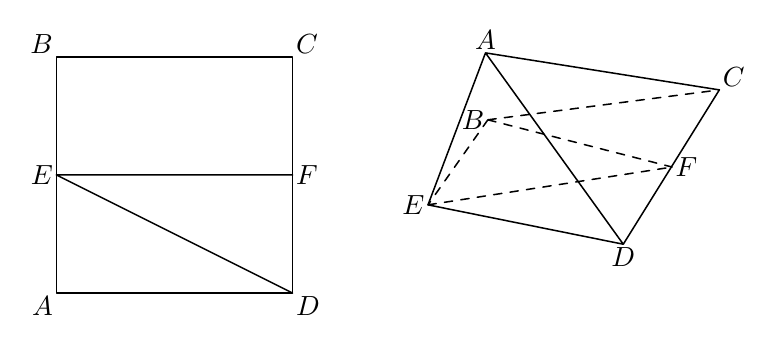
\begin{tikzpicture}[line cap=round,line join=round,line width=0.55pt]
  % Flat square before folding; E and F are the midpoints of AB and CD.
  \coordinate (A0) at (0,0);
  \coordinate (B0) at (0,3);
  \coordinate (C0) at (3,3);
  \coordinate (D0) at (3,0);
  \coordinate (E0) at (0,1.5);
  \coordinate (F0) at (3,1.5);
  \draw (A0)--(B0)--(C0)--(D0)--cycle;
  \draw (E0)--(F0) (E0)--(D0);
  \node[below left,inner sep=1pt] at (A0) {$A$};
  \node[above left,inner sep=1pt] at (B0) {$B$};
  \node[above right,inner sep=1pt] at (C0) {$C$};
  \node[below right,inner sep=1pt] at (D0) {$D$};
  \node[left,inner sep=1pt] at (E0) {$E$};
  \node[right,inner sep=1pt] at (F0) {$F$};

  % Folded view: BCDE is the fixed plane; triangle ADE is rotated about DE.
  \coordinate (A) at (5.45,3.05);
  \coordinate (B) at (5.48,2.20);
  \coordinate (C) at (8.42,2.58);
  \coordinate (D) at (7.20,0.62);
  \coordinate (E) at (4.72,1.12);
  \coordinate (F) at (7.82,1.60);
  \draw[dashed] (B)--(C) (B)--(E) (B)--(F) (E)--(F);
  \draw (C)--(D)--(E) (A)--(E) (A)--(D) (A)--(C);
  \node[above,inner sep=1pt] at (A) {$A$};
  \node[left,inner sep=1pt] at (B) {$B$};
  \node[above right,inner sep=1pt] at (C) {$C$};
  \node[below,inner sep=1pt] at (D) {$D$};
  \node[left,inner sep=1pt] at (E) {$E$};
  \node[right,inner sep=1pt] at (F) {$F$};
\end{tikzpicture}
